% ============================================================
%  Desigualdad del ingreso laboral en Colombia, 2018-2026
%  Formato APA 7 (estudiante) -- compila con pdfLaTeX
%  Overleaf: este archivo, ur.png y fig_*.pdf deben estar en la
%  RAÍZ del proyecto (no dentro de una carpeta). Main document = informe.tex.
%  No necesita biber: las referencias están escritas en el mismo archivo.
%  Las cifras vienen de outputs/*.csv (scripts/correr_todo.R).
% ============================================================
\documentclass[12pt,letterpaper]{article}

% ---------- Idioma y fuentes ----------
\usepackage[T1]{fontenc}
\usepackage[utf8]{inputenc}
\usepackage[spanish,es-nodecimaldot,es-nolists,es-noshorthands]{babel}
\usepackage{amsmath}
\usepackage{mathptmx}            % Times New Roman, como pide la guía (liviano: compila rápido)
\renewcommand{\ttdefault}{lmtt}   % letra de máquina vectorial (Latin Modern)
\usepackage{icomma}            % permite escribir 0,05 en modo matemático
\usepackage{graphicx}          % logo de la portada y figuras

% ---------- Página APA ----------
\usepackage[margin=1in]{geometry}
\usepackage{setspace}
\onehalfspacing
\setlength{\emergencystretch}{1em}   % evita líneas que se salen del margen
\setlength{\parindent}{0.5in}
\setlength{\parskip}{0pt}
\setlength{\textfloatsep}{12pt plus 2pt minus 4pt}   % menos espacio alrededor de tablas y figuras
\setlength{\intextsep}{10pt plus 2pt minus 4pt}
\setlength{\floatsep}{10pt plus 2pt minus 2pt}

\usepackage{fancyhdr}
\pagestyle{plain}
\fancyhf{}
\fancyhead[R]{\thepage}
\renewcommand{\headrulewidth}{0pt}
\setlength{\headheight}{15pt}

% ---------- Títulos APA (sin numeración) ----------
\usepackage{titlesec}
\setcounter{secnumdepth}{0}
% Nivel 1: centrado, negrita
\titleformat{\section}[block]{\normalfont\bfseries\centering}{}{0pt}{}
\titlespacing*{\section}{0pt}{0pt}{0pt}
% Nivel 2: alineado a la izquierda, negrita
\titleformat{\subsection}[block]{\normalfont\bfseries}{}{0pt}{}
\titlespacing*{\subsection}{0pt}{0pt}{0pt}

% ---------- Listas, tablas y enlaces ----------
\usepackage{enumitem}
\setlist{nosep}
\usepackage{array,booktabs}
\usepackage{xurl}
\usepackage[hidelinks]{hyperref}
\urlstyle{same}

% ---------- Tablas y figuras en formato APA ----------
% \apa{Tabla 1}{Título}{contenido}{nota}
\newcommand{\apa}[4]{%
  \singlespacing\raggedright
  {\bfseries #1\par}\vspace{0.4\baselineskip}
  {\itshape #2\par}\vspace{0.4\baselineskip}
  #3\par\vspace{0.3\baselineskip}
  {\small {\itshape Nota.} #4\par}}

% ---------- Referencias APA 7 (escritas a mano: no se necesita biber) ----------
\newenvironment{referencias}{\begin{list}{}{\setlength{\leftmargin}{0.5in}\setlength{\itemindent}{-0.5in}\setlength{\itemsep}{0pt}\setlength{\parsep}{0pt}}\raggedright}{\end{list}}

\newcommand{\titulo}{¿Cómo estimar el índice de Theil con la GEIH? Comparación de cuatro estimadores aplicada a la desigualdad del ingreso laboral en Colombia, 2018--2026}

% ============================================================
\begin{document}

% ---------------- Portada ----------------
\begin{titlepage}
  \thispagestyle{empty}
  \centering
  \singlespacing
  \vspace*{0.2in}
  
\includegraphics[width=2.4in]{ur.png}\par
  \vspace{0.9in}
  \rule{0.75\textwidth}{0.4pt}\par
  \vspace{0.3in}
  {\large\bfseries \titulo\par}
  \vspace{0.3in}
  \rule{0.75\textwidth}{0.4pt}\par
  \vspace{0.9in}
  Gabriel Salcedo\par
  Jerónimo Marín\par
  Isaac Suarez\par
  Santiago Velandia\par
  \vfill
  Universidad del Rosario\par
  \vspace{0.15in}
  Estadística\par
  \vspace{0.15in}
  Noviembre de 2026\par
  \vspace*{0.2in}
\end{titlepage}
\setcounter{page}{2}

% ============================================================
\section{Introducción}

\subsection{Justificación}

Colombia es uno de los países más desiguales de América Latina: en 2024 el Gini del ingreso de los hogares fue 0,551 (DANE, 2025). Pero esa cifra, como cualquier medida de desigualdad, sale de una encuesta. Es una estimación, no el valor real, y el resultado depende de cómo se estime.

Trabajamos con el índice de Theil porque, además de medir la desigualdad, se divide exactamente en dos partes: la desigualdad \emph{entre} grupos y la desigualdad \emph{dentro} de ellos (Shorrocks, 1980). El problema es que con los mismos datos hay varias formas de estimarlo: con o sin los factores de expansión de la encuesta, o suponiendo que el ingreso sigue una distribución lognormal. Cada forma tiene supuestos distintos y, si se elige mal, el resultado queda sesgado.

Por eso hicimos el trabajo en dos pasos. Primero, con un experimento de simulación, comparamos cuatro estimadores del Theil y elegimos el mejor. Después, usamos ese estimador para medir y explicar la desigualdad del ingreso laboral en Colombia entre 2018 y 2026.

\subsection{Estado del arte}

Theil (1967) propuso un índice que vale cero cuando todos ganan lo mismo y crece cuando el ingreso se concentra, y que se descompone por grupos. Efron y Tibshirani (1993) desarrollaron el bootstrap para medir la incertidumbre de un estimador, y Mills y Zandvakili (1997) lo aplicaron a índices de desigualdad: diferencias aparentes entre grupos pueden no ser significativas. Para Colombia, Sánchez-Torres (2017) encontró que cerca del 88~\% de la desigualdad ocurre dentro de los departamentos, y Ariza y Montes-Rojas (2017), que la informalidad aumenta la desigualdad del ingreso laboral. Estos trabajos usan un solo estimador sin justificarlo, estudian un factor a la vez y no reportan la precisión de sus resultados. Nosotros primero validamos el estimador y después lo aplicamos, con cinco dimensiones e intervalos de confianza.

\section{Pregunta problema}

\begin{quote}
\emph{De cuatro estimadores candidatos del índice de Theil ---ponderado (A), sin ponderar (B), lognormal por momentos (C) y lognormal por máxima verosimilitud (D)---, ¿cuál tiene mejores propiedades estadísticas (menor sesgo, menor ECM y consistencia) para estimar la desigualdad del ingreso laboral a partir de la GEIH?}
\end{quote}

\section{Objetivos}

\textbf{General.} Comparar las propiedades estadísticas de cuatro estimadores del índice de Theil mediante un experimento de simulación con la GEIH, y aplicar el estimador validado para medir y explicar la desigualdad del ingreso laboral en Colombia entre 2018 y 2026.

\textbf{Específicos.} (1) Definir los cuatro estimadores (A, B, C y D), sus supuestos y sus propiedades esperadas (sesgo, consistencia, eficiencia y suficiencia). (2) Construir con la GEIH 2024 completa un valor de referencia del Theil contra el cual evaluarlos. (3) Simular submuestras de distintos tamaños para estimar el sesgo, la varianza, el ECM y la eficiencia relativa de cada estimador. (4) Determinar cuál es consistente y debe usarse en el análisis aplicado. (5) Construir bases anuales comparables (enero--junio, 2018--2026) y calcular con el estimador validado el Theil de cada año, excepto 2020, y su descomposición en cinco dimensiones. (6) Estimar intervalos de confianza del 95~\% por bootstrap y contrastar las hipótesis H1, H2 y H3.

% ============================================================
\section{Los cuatro estimadores}

Sea $y_i$ el ingreso laboral de la persona $i$ y $w_i$ su factor de expansión, es decir, a cuántas personas de la población representa ($i = 1, \dots, n$). Queremos estimar el índice de Theil de la población de ocupados:
\begin{equation}
  T = \frac{1}{N}\sum_{j=1}^{N} \frac{Y_j}{\mu_Y}\ln\!\left(\frac{Y_j}{\mu_Y}\right),
\end{equation}
donde $N$ es el tamaño de la población, $Y_j$ el ingreso de cada persona y $\mu_Y$ su media. Si todos ganan lo mismo, $T = 0$; cuanto más concentrado está el ingreso, más grande es $T$.

\textbf{A y B: por sustitución.} Aplican la misma fórmula a la muestra. El estimador \textbf{A} usa los factores de expansión, con $W = \sum_i w_i$ y $\hat{\mu}_w = \frac{1}{W}\sum_i w_i y_i$:
\begin{equation}
  \hat{T}_A = \frac{1}{W}\sum_{i=1}^{n} w_i \frac{y_i}{\hat{\mu}_w}\ln\!\left(\frac{y_i}{\hat{\mu}_w}\right).
\end{equation}
El estimador \textbf{B} es la misma fórmula con $w_i = 1$ para todos. Como la GEIH no le da a todas las personas la misma probabilidad de ser encuestadas, B mide la desigualdad \emph{de los encuestados}, no la de la población, y esperamos que esté sesgado aunque la muestra sea muy grande.

\textbf{C y D: lognormales.} Si $\ln y \sim N(m, \sigma^2)$, entonces $T = \sigma^2/2$ (Cowell, 2011), así que basta con estimar $\sigma^2$:
\begin{equation}
  \hat{T}_C = \frac{1}{2}\ln\!\left(1 + \frac{s_y^2}{\bar{y}^{\,2}}\right),
  \qquad
  \hat{T}_D = \frac{1}{2}\cdot\frac{1}{n}\sum_{i=1}^{n}\left(\ln y_i - \overline{\ln y}\right)^2 .
\end{equation}
C despeja $\sigma^2$ igualando la media y la varianza de la muestra con las de una lognormal (método de los momentos). D usa el estimador de máxima verosimilitud de $\sigma^2$, que divide por $n$ y depende de los datos solo a través de $\sum \ln y_i$ y $\sum (\ln y_i)^2$, sus estadísticos suficientes. C y D no usan factores de expansión. Si el ingreso no es lognormal, esperamos que ambos queden sesgados.

% ============================================================
\section{Datos}

\subsection{Fuente y variables}

Usamos la \textbf{Gran Encuesta Integrada de Hogares (GEIH)} del Departamento Administrativo Nacional de Estadística (DANE, 2026): una encuesta mensual, probabilística y nacional, con cerca de 315.000 hogares al año (DANE, 2023). Es la única fuente que tiene a la vez el ingreso laboral y los factores de expansión; sin estos no se puede construir el estimador A. Para cada año unimos los meses de enero a junio de tres módulos (ocupados, características generales y vivienda). Así obtuvimos nueve bases anuales, de 2018 a 2026, cada una con más de 140.000 ocupados y las 12 variables de la Tabla 1.

\begin{table}[!htb]
\apa{Tabla 1}{Variables de la GEIH usadas en el proyecto}{%
  \small\renewcommand{\arraystretch}{1.0}
  \begin{tabular}{@{}>{\raggedright\arraybackslash}p{1.55in}>{\raggedright\arraybackslash}p{1.55in}>{\raggedright\arraybackslash}p{1.3in}>{\raggedright\arraybackslash}p{1.6in}@{}}
    \toprule
    Variable & Código GEIH & Tipo y escala & Uso \\
    \midrule
    Ingreso laboral mensual & INGLABO & Continua, razón & Cálculo del Theil \\
    Factor de expansión & FEX\_C\_2011 / FEX\_C18 & Continua, razón & Ponderación (A) \\
    Nivel educativo & P6210 / P3042 & Cualitativa, ordinal & Dimensión \\
    Cotización a pensión & P6920 & Cualitativa, nominal & Formalidad (dimensión) \\
    Estrato & P4030S1A1 & Cualitativa, ordinal & Dimensión \\
    Departamento & DPTO & Cualitativa, nominal & Región (dimensión) \\
    Sexo & P6020 / P3271 & Cualitativa, nominal & Dimensión \\
    Posición ocupacional & P6430 & Cualitativa, nominal & Filtro y ajuste de pesos \\
    Edad & P6040 & Discreta, razón & Filtro ($\geq$ 15 años) \\
    Zona & CLASE & Cualitativa, nominal & Descripción \\
    Horas trabajadas & P6800 & Discreta, razón & Descripción \\
    Tamaño de la empresa & P6870 / P3069 & Cualitativa, ordinal & Descripción \\
    \bottomrule
  \end{tabular}}{%
  Cuando hay dos códigos, el primero es el del marco muestral antiguo (2018--2021) y el segundo el del Marco 2018 (2022--2026).}
\end{table}

\subsection{Depuración}

Seguimos una regla: \emph{marcar, no borrar}. La base de cada año conserva a todos los ocupados, y cada criterio se guarda como un indicador. Así se puede contar cuántas personas excluye cada paso (Tabla 2). Los criterios son:

\begin{itemize}[leftmargin=0.75in]
  \item \textbf{Edad:} ocupados de 15 años o más.
  \item \textbf{Remunerados:} se excluyen los trabajadores sin remuneración, porque su ingreso laboral es cero por definición.
  \item \textbf{Cobertura común:} los 24 departamentos que la encuesta cubre en todos los años. El Marco 2018 agrega nueve departamentos (San Andrés y los de Orinoquía-Amazonía) que no existen en 2018--2021; quedan fuera para que la serie sea comparable.
  \item \textbf{Ingreso positivo:} se excluyen los ingresos iguales a cero, para que los cuatro estimadores se calculen sobre la misma población: C y D usan logaritmos y $\ln 0$ no está definido.
  \item \textbf{Dimensiones completas:} la persona debe tener información en las cinco dimensiones.
  \item \textbf{No respuesta de ingreso:} quien no reporta su ingreso no se borra. Su peso se reparte entre quienes sí lo reportan dentro de celdas de personas parecidas (posición ocupacional, formalidad, educación, región y sexo), y el total del factor de expansión se conserva.
\end{itemize}

Las cinco dimensiones son: \textbf{educación}, en cinco niveles comunes a los dos marcos (ninguno o preescolar, primaria, secundaria, media y superior); \textbf{formalidad}, formal si cotiza a pensión o ya está pensionado; \textbf{estrato}, de 1 a 6; \textbf{región}, cinco regiones dentro de la cobertura común (Bogotá, Caribe, Oriental, Central y Pacífica), y \textbf{sexo}. El año 2020 no entra al Theil: por la recolección telefónica durante la pandemia falta el ingreso de la mayoría y no se preguntó el estrato. El análisis aplicado usa, entonces, ocho años.

\begin{table}[!htb]
\apa{Tabla 2}{Personas que quedan después de la depuración (enero--junio de cada año)}{%
  \footnotesize\setlength{\tabcolsep}{3.5pt}
  \begin{tabular}{@{}lrrrrrrrrr@{}}
    \toprule
    & 2018 & 2019 & 2020 & 2021 & 2022 & 2023 & 2024 & 2025 & 2026 \\
    \midrule
    Ocupados             & 174.668 & 168.441 & 146.862 & 146.094 & 194.647 & 183.136 & 178.204 & 176.176 & 177.195 \\
    Población de estudio & 162.300 & 156.616 &  96.931 & 136.479 & 168.270 & 160.299 & 156.063 & 154.659 & 155.262 \\
    Entran al Theil      & 141.025 & 151.283 &  57.042 & 129.750 & 160.946 & 157.776 & 152.213 & 153.340 & 154.657 \\
    \% del FEX total     & 82,6 & 87,6 & 46,4 & 86,2 & 85,3 & 88,3 & 86,9 & 89,1 & 89,0 \\
    \bottomrule
  \end{tabular}}{%
  \emph{Población de estudio}: cumple todos los criterios. \emph{Entran al Theil}: además reportan ingreso positivo. \emph{\% del FEX total}: parte de los ocupados del país que representan, antes del ajuste por no respuesta. 2020 no se usa.}
\end{table}

% ============================================================
\section{Hipótesis}

Todas las pruebas son unilaterales con $\alpha = 0,05$.

\textbf{H1. El estimador ponderado (A) es consistente y tiene el menor ECM de los cuatro cuando el tamaño de muestra crece, mientras que B, C y D no convergen al valor verdadero.} Para cada competidor $j$ y $n = 50.000$ se define, en cada réplica, la diferencia de pérdidas $d_j^{(r)} = (\hat{T}_A^{(r)} - T)^2 - (\hat{T}_j^{(r)} - T)^2$, y se contrasta
\begin{equation}
  H_0:\; \bar{d}_j \geq 0 \qquad\qquad H_1:\; \bar{d}_j < 0, \qquad j \in \{B, C, D\}
\end{equation}
con una prueba $t$ pareada sobre las $R$ réplicas. Se concluye a favor de A si se rechaza $H_0$ frente a los tres competidores. La consistencia se evalúa además con la tendencia del ECM a lo largo de los cuatro tamaños de muestra.

\textbf{H2 (aplicada, con el estimador elegido). En 2026 la educación explica más desigualdad que cada una de las otras cuatro dimensiones.} $H_0: S_{edu} \leq S_k$ para algún $k$, frente a $H_1: S_{edu} > S_k$ para todo $k$. Se rechaza $H_0$ si el percentil 5 de cada diferencia bootstrap $S_{edu}^{*b} - S_k^{*b}$ es mayor que cero.

\textbf{H3 (aplicada). La desigualdad del ingreso laboral fue menor en 2026 que en 2018.} $H_0: T_{2026} \geq T_{2018}$ frente a $H_1: T_{2026} < T_{2018}$. Se rechaza $H_0$ si el percentil 95 de las diferencias $T_{2026}^{*b} - T_{2018}^{*b}$ es menor que cero. Además de la decisión reportamos el tamaño de la diferencia, porque con muestras tan grandes casi todo resulta significativo.

% ============================================================
\section{Cómo hicimos el trabajo}

\subsection{Plan de trabajo}

El proyecto avanzó en seis etapas (Tabla 3). Cada etapa es un programa de R que lee lo que produjo la anterior, así que cualquier persona puede repetir el trabajo completo en el mismo orden.

\begin{table}[!htb]
\apa{Tabla 3}{Etapas del proyecto}{%
  \small\renewcommand{\arraystretch}{1.0}
  \begin{tabular}{@{}l>{\raggedright\arraybackslash}p{3.4in}>{\raggedright\arraybackslash}p{1.7in}@{}}
    \toprule
    Etapa & Qué hicimos & Programa de R \\
    \midrule
    1. Extracción & Unir los módulos de la GEIH, enero a junio de cada año & \texttt{01\_extraer\_crudas.R} \\
    2. Depuración & Armonizar variables, marcar criterios y ajustar pesos por no respuesta & \texttt{02\_bases\_finales.R} \\
    3. Descriptiva & Medidas, frecuencias, tablas cruzadas y figuras ponderadas & \texttt{03\_descriptiva.R} \\
    4. Aplicación & Theil por año y descomposición en cinco dimensiones & \texttt{04\_theil\_anual.R} \\
    5. Simulación & Comparar A, B, C y D y probar H1 & \texttt{05\_simulacion.R} \\
    6. Inferencia & Intervalos de confianza bootstrap y pruebas de H2 y H3 & \texttt{06\_bootstrap.R} \\
    \bottomrule
  \end{tabular}}{%
  Las fórmulas de los cuatro estimadores y de la descomposición están en \texttt{00\_funciones.R}; \texttt{correr\_todo.R} ejecuta las etapas 2 a 6 en unos 11 minutos.}
\end{table}

\subsection{El experimento de simulación}

Para comparar los estimadores necesitamos conocer el valor verdadero, y en la vida real no lo conocemos. Por eso tratamos la GEIH 2024 completa como si fuera la población. Hicimos lo siguiente:
\begin{enumerate}[leftmargin=0.75in]
  \item Tomamos las 152.213 personas de 2024 que entran al Theil, con sus pesos, y calculamos el valor de referencia con el estimador A sobre toda la base: $T = 0,5043$.
  \item Elegimos cuatro tamaños de muestra: $n$ = 500, 2.000, 10.000 y 50.000.
  \item Para cada tamaño sacamos 500 submuestras por muestreo aleatorio simple sin reemplazo. Cada persona conservó su factor de expansión.
  \item En cada submuestra calculamos A, B, C y D.
  \item Con los 500 valores de cada estimador calculamos el sesgo (promedio menos $T$), la varianza, el ECM (sesgo$^2$ + varianza) y la eficiencia relativa, $\text{ECM}(A)/\text{ECM}(j)$: si es menor que 1, A tiene menos error que $j$.
\end{enumerate}

\subsection{Bootstrap y herramientas}

Para medir la precisión de cada año usamos bootstrap: remuestreamos personas con reemplazo, el mismo número que tiene la base, cada una con su peso, y en cada una de las 500 réplicas recalculamos el Theil y, en 2026, las cinco descomposiciones. El intervalo de confianza del 95~\% va del percentil 2,5 al 97,5 de las réplicas; H2 y H3 se prueban con los percentiles descritos en la sección de hipótesis. Todo el análisis se hizo en R 4.5.2 con los paquetes \texttt{dplyr} y \texttt{tidyr} (datos), \texttt{ggplot2} y \texttt{scales} (figuras), \texttt{quantreg} (cuantiles ponderados) y \texttt{haven} (lectura de los archivos del DANE). La simulación y el bootstrap usan semillas fijas, así que cada vez que se corre el código salen exactamente los mismos números. El código, los datos depurados y las instrucciones están en \url{https://github.com/gabrielsalcedo/statistics-geih}.

% ============================================================
\section{Estadística descriptiva}

Todas las cifras están ponderadas: describen a los ocupados del país, no a los encuestados. En 2026, las 154.657 personas del análisis representan 21,6 millones de ocupados por mes. Ponderar importa: Bogotá es el 4,4~\% de los encuestados, pero el 19,6~\% de los ocupados. El 57~\% de los ocupados son hombres, el 38~\% tiene educación superior, la mitad es informal (50,6~\%) y dos de cada tres viven en estrato 1 o 2. Las dimensiones van juntas: la informalidad es de 95,2~\% sin educación y de 21,9~\% con educación superior, y en el estrato 6 el 88~\% tiene educación superior, frente al 16,6~\% en el estrato 1. Las brechas son grandes: el ingreso medio del estrato 6 es 4,2 veces el promedio, y quienes tienen educación superior (38~\% de los ocupados) reciben el 60,5~\% del ingreso.

\begin{table}[!htb]
\apa{Tabla 4}{Medidas descriptivas ponderadas de las variables cuantitativas, 2026}{%
  \small\renewcommand{\arraystretch}{1.0}
  \begin{tabular}{@{}lrrrrrr@{}}
    \toprule
    Variable & Media & Mediana & Desv. est. & CV (\%) & Asimetría & Curtosis \\
    \midrule
    Ingreso (\$)   & 2.314.067 & 1.750.000 & 3.083.758 & 133,3 & 9,91  & 198,9 \\
    ln(ingreso)    & 14,24     & 14,38     & 0,95      & 6,6   & $-$0,77 & 4,11 \\
    Edad (años)    & 41,0      & 40        & 13,7      & 33,4  & 0,42  & $-$0,48 \\
    Horas semanales& 43,0      & 44        & 13,0      & 30,2  & 0,05  & 2,57 \\
    \bottomrule
  \end{tabular}}{%
  Ponderado con el factor de expansión ajustado. Curtosis en exceso (0 = normal). Ingreso en pesos corrientes. En 2018 el ingreso tenía media de \$1.057.786, mediana de \$781.242 y CV de 137~\%.}
\end{table}

El ingreso laboral es muy asimétrico (Tabla 4): en 2026 la media (\$2.314.067) está muy por encima de la mediana (\$1.750.000), el coeficiente de variación es 133~\% y la asimetría es 9,9. La Figura 1 muestra un pico en el salario mínimo: el 15,5~\% de los ocupados gana alrededor de un salario mínimo, el 39,5~\% gana menos y solo el 4,3~\% gana más de cuatro. Y el logaritmo del ingreso no es normal: tiene asimetría negativa ($-$0,77) y colas más pesadas que la normal (curtosis en exceso de 4,11). \textbf{Antes de simular, esto ya anticipaba que C y D, que suponen lognormalidad, iban a fallar.}

\begin{figure}[!htb]
\apa{Figura 1}{Distribución del ingreso laboral, 2026}{%
  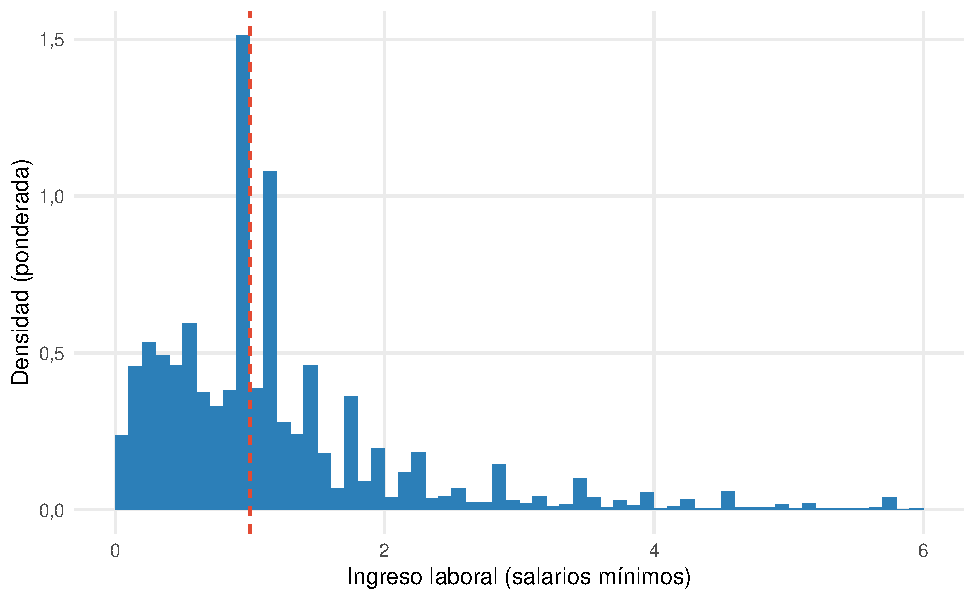
\includegraphics[width=0.53\textwidth]{fig_histograma_ingreso.pdf}}{%
  Densidad ponderada. La línea roja marca 1 salario mínimo (SMMLV). Se muestran los ingresos hasta 6 SMMLV, que cubren el 98,2~\% de los ocupados.}
\end{figure}

% ============================================================
\section{Resultados del experimento}

La Tabla 5 resume las 2.000 submuestras. La conclusión es clara: \textbf{solo A es consistente.} Su sesgo pasa de $-$0,032 con $n = 500$ a casi cero con $n = 50.000$, y su ECM cae sin parar al crecer la muestra (Figura 2).

\begin{table}[!htb]
\apa{Tabla 5}{Sesgo, error cuadrático medio y eficiencia relativa según el tamaño de muestra}{%
  \small\renewcommand{\arraystretch}{1.0}
  \begin{tabular}{@{}lrrrr@{}}
    \toprule
    Estimador & $n = 500$ & $n = 2.000$ & $n = 10.000$ & $n = 50.000$ \\
    \midrule
    \multicolumn{5}{@{}l}{\itshape Sesgo} \\
    A (ponderado)           & $-$0,0321 & $-$0,0095 & $-$0,0020 & 0,0003 \\
    B (sin ponderar)        & $-$0,0847 & $-$0,0795 & $-$0,0775 & $-$0,0766 \\
    C (lognormal, momentos) & $-$0,0275 & 0,0032    & 0,0195    & 0,0243 \\
    D (lognormal, MV)       & $-$0,0773 & $-$0,0777 & $-$0,0778 & $-$0,0780 \\
    \addlinespace
    \multicolumn{5}{@{}l}{\itshape ECM ($\times 10^{3}$)} \\
    A & 23,89 & 7,49 & 1,83 & 0,25 \\
    B & 13,43 & 8,16 & 6,40 & 5,93 \\
    C & 21,95 & 9,87 & 2,98 & 0,97 \\
    D & 7,62  & 6,43 & 6,13 & 6,09 \\
    \addlinespace
    \multicolumn{5}{@{}l}{\itshape Eficiencia relativa: ECM(A) / ECM(j)} \\
    B & 1,78 & 0,92 & 0,29 & 0,04 \\
    C & 1,09 & 0,76 & 0,61 & 0,26 \\
    D & 3,14 & 1,17 & 0,30 & 0,04 \\
    \bottomrule
  \end{tabular}}{%
  500 réplicas por tamaño; valor de referencia $T = 0,5043$. Una eficiencia relativa menor que 1 indica que A tiene menor ECM que el competidor.}
\end{table}

Los demás fallan por razones distintas. \textbf{B y D convergen a un valor equivocado}, cerca de 0,427, un 15~\% por debajo del valor de referencia: B por ignorar el factor de expansión y D por suponer que el ingreso es lognormal. \textbf{C también queda sesgado}, pero hacia arriba ($+$0,024, cerca de un 5~\%). Más datos no corrigen ninguno de estos sesgos.

Hay un matiz: \textbf{con muestras pequeñas A no es el mejor}. Con $n = 500$, D tiene un ECM tres veces menor porque casi no varía, aunque esté sesgado; A subestima porque una submuestra pequeña rara vez incluye los pocos ingresos muy altos. Desde $n = 10.000$ gana A, y con $n = 50.000$ su error es entre 4 y 24 veces menor. Como cada año de la GEIH tiene más de 129.000 personas, \textbf{en la aplicación usamos A}.

\begin{figure}[!htb]
\apa{Figura 2}{Error cuadrático medio de cada estimador según el tamaño de muestra}{%
  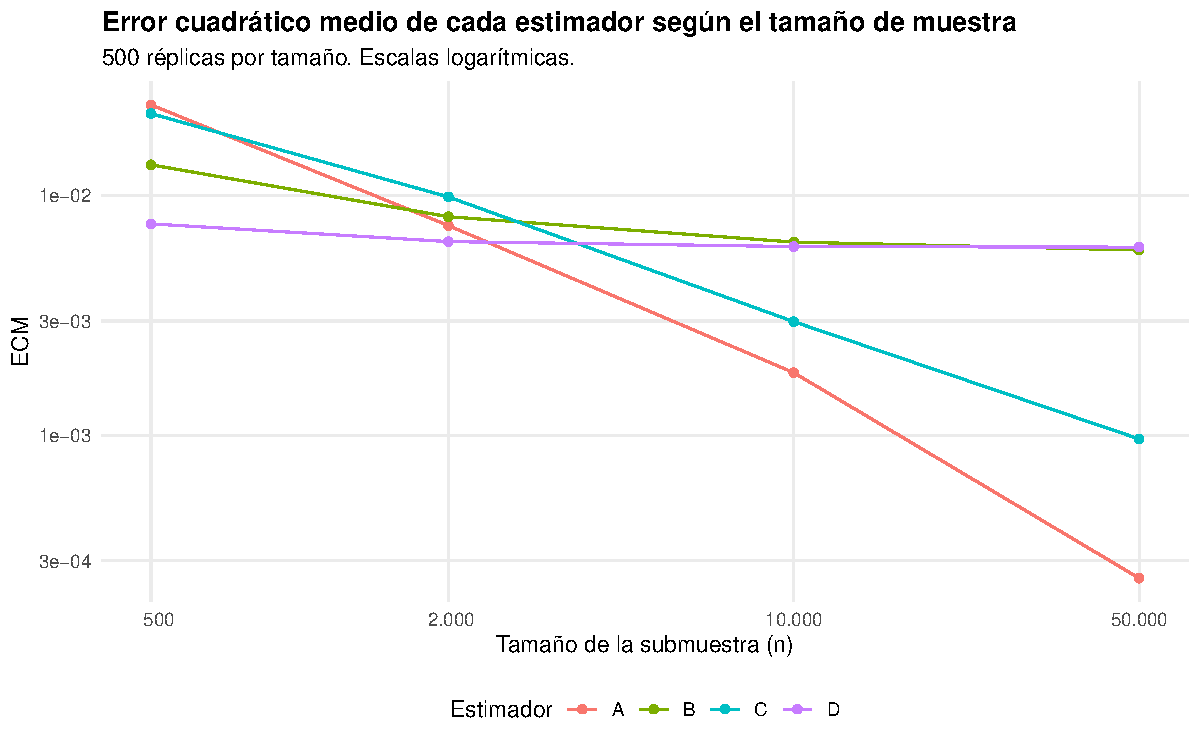
\includegraphics[width=0.53\textwidth]{fig_simulacion_ecm.pdf}}{%
  500 réplicas por tamaño. Ambos ejes en escala logarítmica; el ECM está multiplicado por 1.000, como en la Tabla 5.}
\end{figure}

% ============================================================
\section{Desigualdad del ingreso laboral, 2018--2026}

Con el estimador A, la desigualdad subió de 0,439 en 2018 a 0,477 en 2019 y llegó a su máximo en 2022 (0,538). Desde entonces bajó cada año, hasta 0,429 en 2026, el valor más bajo de la serie (Tabla 6). El salto de 2022 coincide con el cambio del marco muestral y del factor de expansión, así que parte puede ser metodológico. En todos los años B es entre 0,04 y 0,08 menor que A: con datos reales se repite lo que vimos en la simulación. El ajuste por no respuesta mueve poco el resultado (columna \emph{A sin ajuste}).

\begin{table}[!htb]
\apa{Tabla 6}{Índice de Theil del ingreso laboral por año}{%
  \small\renewcommand{\arraystretch}{1.0}
  \begin{tabular}{@{}lrcrr@{}}
    \toprule
    Año & A (principal) & IC 95~\% bootstrap & A sin ajuste & B (sin pesos) \\
    \midrule
    2018 & 0,4392 & [0,4220; 0,4553] & 0,4322 & 0,3891 \\
    2019 & 0,4772 & [0,4597; 0,4955] & 0,4733 & 0,4126 \\
    2021 & 0,4739 & [0,4540; 0,4968] & 0,4622 & 0,4150 \\
    2022 & 0,5381 & [0,5097; 0,5725] & 0,5314 & 0,4536 \\
    2023 & 0,5135 & [0,4932; 0,5345] & 0,5083 & 0,4382 \\
    2024 & 0,5043 & [0,4842; 0,5257] & 0,4981 & 0,4273 \\
    2025 & 0,4609 & [0,4426; 0,4804] & 0,4576 & 0,3916 \\
    2026 & 0,4288 & [0,4124; 0,4459] & 0,4279 & 0,3921 \\
    \bottomrule
  \end{tabular}}{%
  A: con el factor de expansión ajustado por no respuesta. A sin ajuste: con el factor original. B: sin factor. Intervalos por bootstrap de personas (500 réplicas).}
\end{table}

¿Qué explica la desigualdad? \textbf{El estrato es la dimensión que más explica} en todos los años: entre 31~\% y 38~\% del Theil. Le siguen la educación (24--27~\%) y la formalidad (22--27~\%), casi a la par; la región explica entre 5~\% y 9~\%, y el sexo, menos del 1~\% (Figura 3). Aun así, \textbf{la mayor parte de la desigualdad ocurre dentro de los grupos}: incluso con el estrato, unos dos tercios de la desigualdad se dan entre personas del mismo estrato. Como las dimensiones están relacionadas entre sí, sus porcentajes no se suman.

\begin{figure}[!htb]
\apa{Figura 3}{Porcentaje de la desigualdad explicado por cada dimensión (componente entre)}{%
  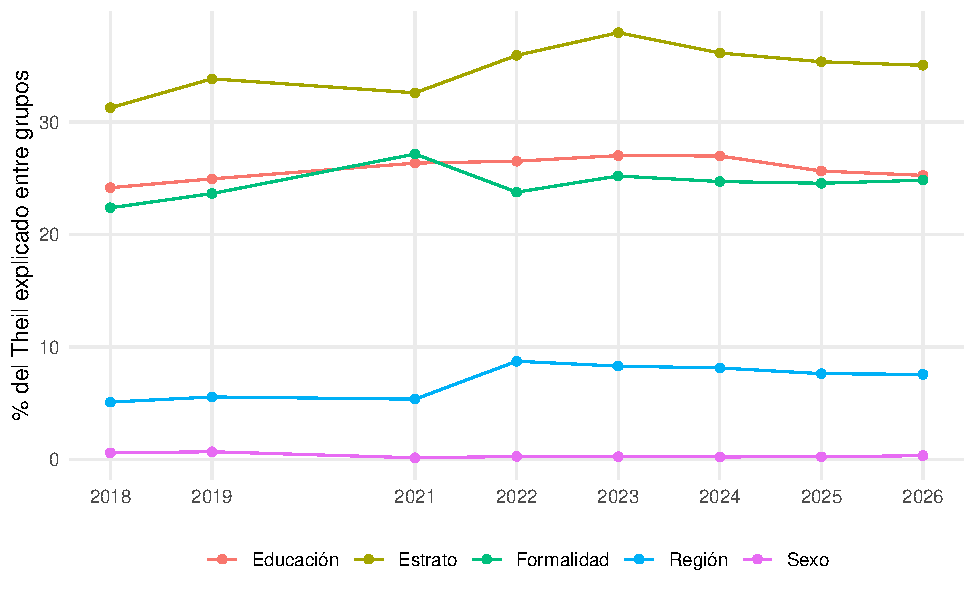
\includegraphics[width=0.53\textwidth]{fig_descomposicion.pdf}}{%
  Porcentaje del índice de Theil (estimador A) que explican las diferencias entre los grupos de cada dimensión.}
\end{figure}

% ============================================================
\section{Pruebas de hipótesis}

\textbf{H1: se cumple.} En cada una de las 500 réplicas con $n = 50.000$ calculamos $d_j = (\hat{T}_A - T)^2 - (\hat{T}_j - T)^2$ y aplicamos una prueba $t$ pareada unilateral con 499 grados de libertad. La media de $d_j$ es negativa frente a los tres competidores: $-$0,00567 frente a B ($t = -109,41$), $-$0,00071 frente a C ($t = -14,89$) y $-$0,00584 frente a D ($t = -219,18$), todos con $p < 0,001$. Se rechaza $H_0$: con muestras grandes, A tiene un ECM significativamente menor. Como el número de réplicas lo elige el investigador, lo que importa es el tamaño de la diferencia: la eficiencia relativa (Tabla 5).

\textbf{H2: no se cumple.} Con las 500 réplicas bootstrap de 2026, la educación explica más que el sexo (percentil 5 de $S^*_{edu} - S^*_k$: 0,235) y que la región (0,165), pero empata con la formalidad (percentil 5: $-$0,003) y explica unos 10 puntos menos que el estrato ($-$0,113). Como el percentil 5 no es positivo frente a todas las dimensiones, no se rechaza $H_0$.

\textbf{H3: no se cumple.} El Theil de 2026 (0,4288) es 0,010 menor que el de 2018 (0,4392), pero el percentil 95 de $T^*_{2026} - T^*_{2018}$ es 0,0085, mayor que cero. No se rechaza $H_0$: la reducción no es significativa y los intervalos de los dos años se superponen (Tabla 6). En cambio, dentro del mismo marco muestral, la caída entre 2022 (0,538) y 2026 (0,429) es grande y los intervalos no se superponen.

% ============================================================
\section{Discusión}

Nuestros resultados coinciden con la literatura y la amplían. Como Sánchez-Torres (2017), que encontró que el 88~\% de la desigualdad ocurre dentro de los departamentos, nosotros encontramos que la región explica solo entre 5~\% y 9~\%: la desigualdad está sobre todo dentro de los territorios. Como Ariza y Montes-Rojas (2017), encontramos que la informalidad pesa: la formalidad explica entre 22~\% y 27~\% del Theil. Y como advierten Mills y Zandvakili (1997), una diferencia que se ve a simple vista puede no ser significativa: es lo que pasa con la caída entre 2018 y 2026. Lo que agregamos es la validación previa: el estimador importa, y B, C o D habrían errado la medida sin importar cuántos datos se tuvieran.

\textbf{Limitaciones.} (1) El valor de referencia es el propio A sobre la GEIH 2024, no la población real. (2) Los factores de expansión y el cuestionario cambiaron en 2022; parte de las diferencias entre años puede ser metodológica. (3) El bootstrap remuestrea personas e ignora que la encuesta selecciona grupos de hogares, así que los intervalos pueden quedar algo estrechos. (4) La no respuesta de ingreso es mayor en los estratos altos y el ajuste no usa el estrato, lo que puede subestimar la desigualdad de 2018. (5) Desde 2022, unos 3.400 ocupados por año figuran como ``sin remuneración'' pero reportan ingreso; seguimos la clasificación del DANE y quedaron fuera. (6) Los ingresos altos suelen subreportarse, y los resultados muestran asociación, no causalidad.

\textbf{Consideraciones éticas.} Los microdatos de la GEIH son públicos y anónimos; no identificamos a ninguna persona ni hogar. Como las cifras de desigualdad orientan la política pública, una estimación sesgada puede llevar a decisiones equivocadas. Por eso reportamos cada estimación con su intervalo de confianza, explicamos las limitaciones, no presentamos asociaciones como causas y dejamos el código y los datos depurados abiertos para que cualquiera pueda verificar el trabajo.

% ============================================================
\section{Conclusiones}

\begin{enumerate}[leftmargin=0.75in]
  \item \textbf{Con la GEIH hay que usar el estimador ponderado (A).} Es el único consistente. Ignorar el factor de expansión (B) o suponer que el ingreso es lognormal (C y D) deja sesgos de 5~\% a 15~\% que no desaparecen con más datos.
  \item \textbf{El supuesto lognormal falla} porque el ingreso laboral tiene un pico en el salario mínimo y colas pesadas.
  \item \textbf{La desigualdad subió hasta 2022 y desde entonces bajó cada año}, hasta su mínimo en 2026; aun así, la diferencia con 2018 no es significativa (H3).
  \item \textbf{El estrato es lo que más explica la desigualdad}; la educación y la formalidad empatan detrás (H2 no se cumple). La mayor parte de la desigualdad ocurre dentro de los grupos.
\end{enumerate}

La lección de método: antes de medir, hay que validar cómo se mide. Sin el experimento habríamos podido reportar una desigualdad un 15~\% menor sin darnos cuenta.

% ---------------- Referencias ----------------
\clearpage
\section{Referencias}

\begin{referencias}
  \item Ariza, J., y Montes-Rojas, G. (2017). Labour income inequality and the informal sector in Colombian cities. \emph{Cuadernos de Economía, 36}(72), 77--98. \url{https://doi.org/10.15446/cuad.econ.v36n72.65820}
  \item Cowell, F. A. (2011). \emph{Measuring inequality} (3.ª ed.). Oxford University Press.
  \item Departamento Administrativo Nacional de Estadística. (2023). \emph{Metodología general Gran Encuesta Integrada de Hogares -- GEIH} (DSO-GEIH-MET-001, versión 11). DANE. \url{https://www.dane.gov.co/files/operaciones/GEIH/met-GEIH.pdf}
  \item Departamento Administrativo Nacional de Estadística. (2025). \emph{Pobreza monetaria en Colombia: año 2024} [Boletín técnico]. DANE. \url{https://www.dane.gov.co/files/operaciones/PM/bol-PM-2024.pdf}
  \item Departamento Administrativo Nacional de Estadística. (2026). \emph{Gran Encuesta Integrada de Hogares -- GEIH, 2018--2026} [Conjunto de datos]. DANE. \url{https://microdatos.dane.gov.co}
  \item Efron, B., y Tibshirani, R. J. (1993). \emph{An introduction to the bootstrap}. Chapman \& Hall. \url{https://doi.org/10.1201/9780429246593}
  \item Mills, J. A., y Zandvakili, S. (1997). Statistical inference via bootstrapping for measures of inequality. \emph{Journal of Applied Econometrics, 12}(2), 133--150.
  \item Sánchez-Torres, R. M. (2017). Desigualdad del ingreso en Colombia: un estudio por departamentos. \emph{Cuadernos de Economía, 36}(72), 139--178. \url{https://doi.org/10.15446/cuad.econ.v36n72.65880}
  \item Shorrocks, A. F. (1980). The class of additively decomposable inequality measures. \emph{Econometrica, 48}(3), 613--625. \url{https://doi.org/10.2307/1913126}
  \item Theil, H. (1967). \emph{Economics and information theory}. North-Holland.
\end{referencias}

\end{document}
